%\documentclass[10pt,handout,compress,professionalfont]{beamer}
\documentclass[10pt,compress,professionalfont]{beamer}



\usepackage[latin1]{inputenc}
\usepackage{graphicx}
%\usepackage{pgf}

\usepackage{pstricks} 
\usepackage{pstricks-add} 
\usepackage{pst-plot} 
\usepackage{pst-text,pst-node,pst-tree} 




%\hypersetup{pdfstartview={FitH}}


\setbeamertemplate{navigation symbols}{}
%\usetheme{Warsaw}
\usecolortheme{beaver}
\usefonttheme{structuresmallcapsserif}



\usepackage{beamerthemeAmsterdam} 



\title[Point-Based Color Bleeding With Volumes]{PCBEX:\\An Approach to Point-Based Color Bleeding With Volumes}
\author{Christopher James Gibson\thanks{e-mail: cgibson@calpoly.edu}\\
\and Zo\"{e} J. Wood\thanks{e-mail: zwood@calpoly.edu}}
\institute{California Polytechnic State University\\San Luis Obispo\\CSC Department}
\date{June 9, 2011}

\setcounter{tocdepth}{1}

\begin{document}

\AtBeginSection[]
{
  \begin{frame}<beamer>
    \frametitle{Outline}

    \begin{columns}
        \begin{column}{0.65\textwidth}
            \tableofcontents[currentsection,currentsubsection,hideallsubsections]
        \end{column}
        \begin{column}{0.35\textwidth}
                \vspace{-9mm}
                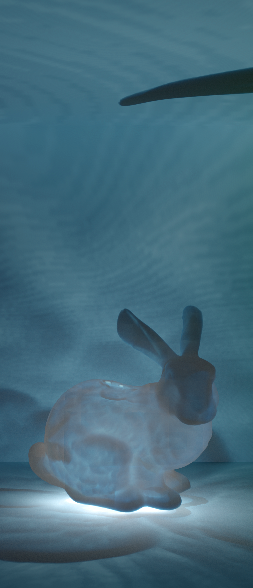
\includegraphics[height=90mm]{../img/bunny_glow_crop2}
        \end{column}
    \end{columns}
  \end{frame}
}




%%----------------------------------------------------------------------  TITLE
\begin{frame}

    \titlepage

\end{frame}


%%------------------------------------------  RELATED WORK: GLOBAL ILLIMUNATION
\begin{frame}{Outline}

    \begin{columns}
        \begin{column}{0.5\textwidth}

            \vspace{-4mm}
            \begin{itemize}
                \item Background\\ \vspace{2mm}
                \item Motivation and Goals\\ \vspace{2mm}
                \item Algorithm Details\\ \vspace{2mm}
                \item Results
            \end{itemize}
        \end{column}
        \begin{column}{0.5\textwidth}
            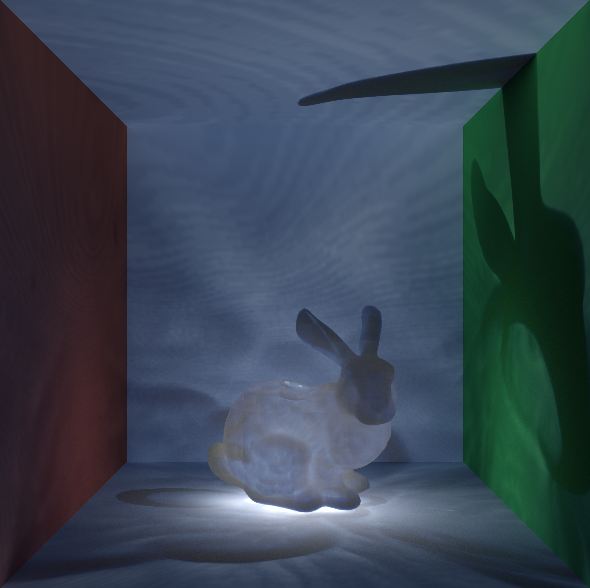
\includegraphics[width=\textwidth]{../img/bunny_glow}
        \end{column}
    \end{columns}

\end{frame}




%\section{Background}
\subsection{GI Techniques}
%\subsection{Global Illumination}
%%--------------------------------------------  BACKGROUND: GLOBAL ILLIMUNATION
\begin{frame}{Global Illumination}

    \begin{columns}
        \begin{column}{0.55\textwidth}
	    Light's interaction with various materials and mediums is complex and beautiful\\
	    \vspace{6mm}
	    Light does not simply hit surfaces, but bounces and passes through them as well\\
            \vspace{6mm}
            Global Illumination Algorithms attempt to evaluate/approximate these interactions\\
        \end{column}
        \begin{column}{0.45\textwidth}
            {\centering
                \vspace{-4mm}
                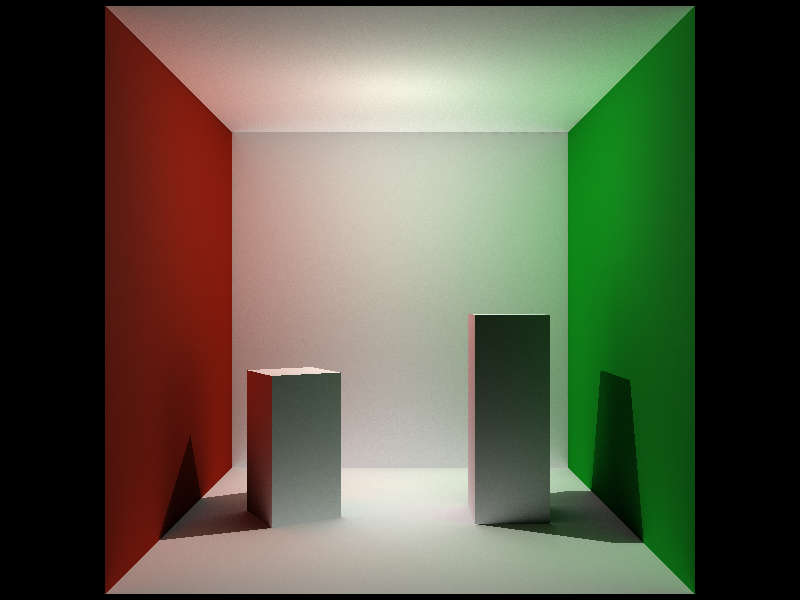
\includegraphics[width=\textwidth]{../img/indirect_box_high}
            }
        \end{column}
    \end{columns}

\end{frame}




%\subsection{Point-Based Color Bleeding}
%%------------------------------------------------  BACKGROUND: VOLUME LIGHTING
\begin{frame}{Point-Based Color Bleeding (PCB)}


    \begin{columns}
        \begin{column}{0.65\textwidth}
            Cheap, approximate global illumination effects using color bleeding\\
            \vspace{8mm}
            Utilizes direct light point cloud representation of scene's direct lighting\\
            \vspace{8mm}
            Already used heavily in production due to its performance advantages

        \end{column}
        \begin{column}{0.35\textwidth}
            {\centering
                \vspace{-4mm}
                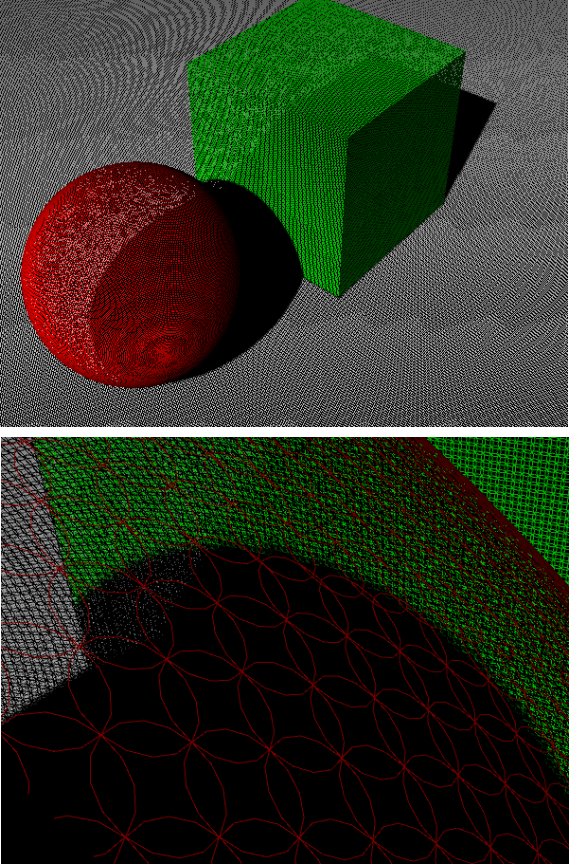
\includegraphics[width=\textwidth]{../img/external/pcb}\\
                \scriptsize Surfels in PCB\\\textit{(image source: Per Christensen)}
            }
        \end{column}
    \end{columns}

\end{frame}


%%\section{PCB Extension Algorithm}
%\subsection{PCB Algorithm Overview}
%%--------------------------------------------------------------  PCB EXTENSION
\begin{frame}{Point-Based Color Bleeding (PCB)}

    \begin{columns}
        \begin{column}{0.6\textwidth}
            \begin{enumerate}
                \item Sample the scene and generate a point cloud
                \item Perform normal ray tracing
                \item Replace ambient estimates with a gather stage using surrounding point cloud
            \end{enumerate}
        \end{column}
        \begin{column}{0.4\textwidth}
            {\centering
                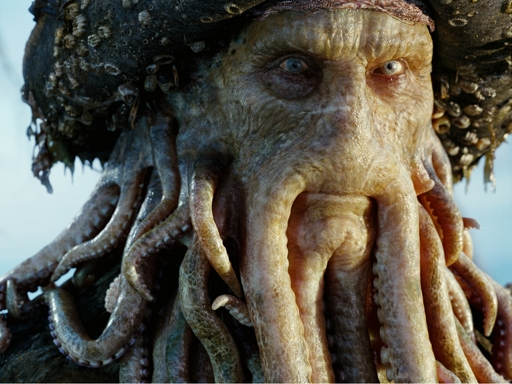
\includegraphics[width=\textwidth]{../img/external/davyjones}\\
                \centering{\scriptsize\textit{(image source: Disney)}}
            }
        \end{column}
    \end{columns}
\end{frame}


\subsection{Light}
%%---------------------------------------------------  BACKGROUND: ILLIMUNATION
\begin{frame}{Irradiance and Radiance}

    \begin{columns}
        \begin{column}{0.5\textwidth}
                \begin{block}{Irradiance Equation}
                    \[
                    E = \frac{d\Phi}{dA}
                    \]
                \end{block}
            \begin{block}{Radiance Equation}
                \[
                \mathit{L} = \frac{\mathit{d^{2}\Phi}}{\mathit{dw\:dA}^\perp} = \frac{\mathit{d^{2}\Phi}}{\mathit{dw\:dA}\textup{cos}\theta}
                \]
            \end{block}
            \begin{block}{Radiance Invariance}
                \[
                    L(x \to y) = L(y \to x)
                \]
            \end{block}
        \end{column}
        \begin{column}{0.5\textwidth}
            \vspace{-5mm}
            {\centering
            \includegraphics[width=\textwidth]{../img/diag/radiance.pdf}\\
            \scriptsize Radiance diagram\\
            }
        \end{column}
    \end{columns}


        % NOTE: Flux density per unit area, per unit solid angle
        % NOTE: dA is the projection of dA on a plane perpendicular to w
        % NOTE: radiance is incoming light power

\end{frame}



\subsection{Light \& Volumes}
%\subsection{Volume Lighting}
%%---------------------------------------------------  BACKGROUND: ILLIMUNATION
\begin{frame}{Volume Lighting}

    \centering
    \vspace{0cm}
    \includegraphics[width=100mm]{../img/diag/vol_scatter.pdf}

\end{frame}


%%---------------------------------------------------  BACKGROUND: ILLIMUNATION
\begin{frame}{Volume Lighting- Scatter, Absorption and Transmittance}


    \begin{columns}
        \begin{column}{0.5\textwidth}

            \begin{block}{Absorption Equation}
                \[
                    e^{-\int_{0}^{d}\sigma_{a} (p+t\mathit{w},\mathit{w})d\mathit{t}}
                \]
            \end{block}

            \begin{block}{Scatter Out Equation}
                \[
                    d\mathit{L}_{o}(\textup{p},w) = -\sigma_{s}(\textup{p},w) \mathit{L}_{i}(\textup{p},-w)dt
                \]
            \end{block}

            \begin{block}{Transmittance Equation}
                \[
                    T_{r}(\textup{p} \to \textup{p}') = e^{-\int_{0}^{d}\sigma (p+t\mathit{w},\mathit{w})d\mathit{t}}.
                \]
            \end{block}

        \end{column}
        \begin{column}{0.5\textwidth}
            \vspace{10mm}
            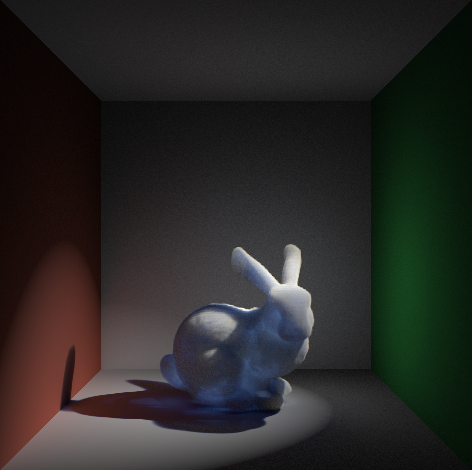
\includegraphics[width=\textwidth]{../img/bunny_spot/spot_right_new}
        \end{column}
    \end{columns}

\end{frame}




%%---------------------------------------------------  BACKGROUND: ILLIMUNATION
\begin{frame}{Volume Lighting - Scatter-In}

    \begin{block}{Scatter-In Equation}
        \[
            \mathit{S}(\textup{p},w) = \mathit{L}_{\textup{ve}}(\textup{p},w) + \sigma_{\textup{s}}(\textup{p}, w) \int_{\mathbb{S}^2} phase(\textup{p}, -w' \to w) L_{i}(\textup{p},w')\textup{d}w'.
        \]
    \end{block}
    {\centering
    \vspace{8mm}
    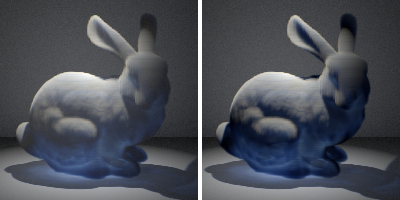
\includegraphics[width=60mm]{../img/inscat_comp}\\
    {\centering\scriptsize Scatter-in \textit{(left)} and only direct lighting via transmittance \textit{(right)}\\}
    }

\end{frame}



%\section{Algorithm}
\subsection{Motivation & Gloals}
%%------------------------------------------  RELATED WORK: GLOBAL ILLIMUNATION
\begin{frame}{Motivation}

    \begin{columns}
        \begin{column}{0.35\textwidth}
            {\centering 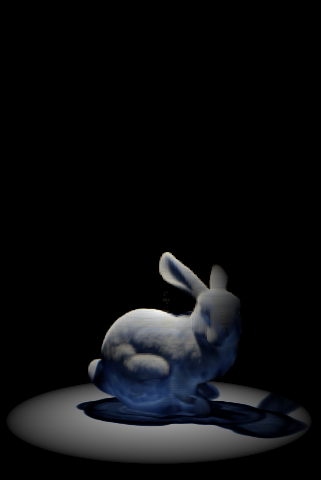
\includegraphics[width=\textwidth]{../img/bunny_spot_sad}\\}

        \end{column}
        \begin{column}{0.65\textwidth}
            Complex volume lighting algorithms are computationally expensive and complex\\
            \vspace{8mm}
            Most GI algorithms do not include volume contributions\\
            
        \end{column}
    \end{columns}
\end{frame}



%%------------------------------------------  RELATED WORK: GLOBAL ILLIMUNATION
\begin{frame}{Goals}

    \begin{columns}
        \begin{column}{0.5\textwidth}

            \vspace{-4mm}
            \begin{itemize}
                \item Modify existing PCB in order to include volumetric lighting\\ \vspace{2mm}
                \item Accurately model scatter, absorption and lighting properties\\ \vspace{2mm}
                \item Modify volume integration algorithm to add scatter-in effects\\ \vspace{2mm}
                \item Return comparable results with shorter overall runtimes
            \end{itemize}
        \end{column}
        \begin{column}{0.5\textwidth}
            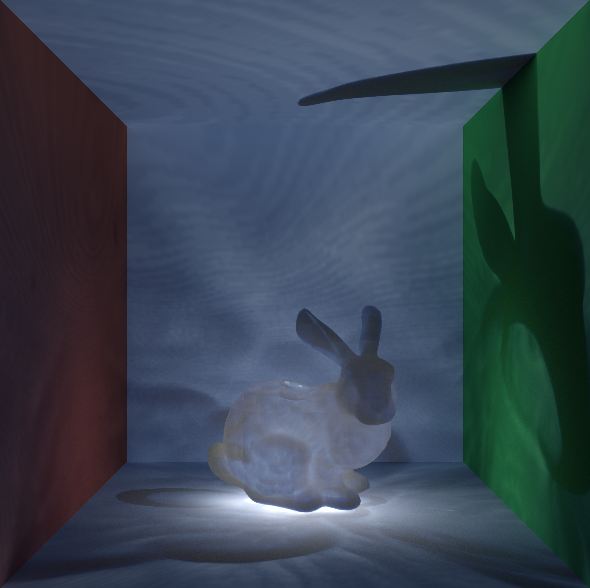
\includegraphics[width=\textwidth]{../img/bunny_glow}
        \end{column}
    \end{columns}

\end{frame}




\subsection{Algorithm Extension Overview}
%\subsection{Extension Overview}
%%--------------------------------------------------------------  PCB EXTENSION
\begin{frame}{Extension Overview}

    \begin{enumerate}
        \item Sample the scene and generate a point cloud
        \item \alert{ Sample the participating media to evaluate scatter, absorbtion and direct lighting}
        \item Perform normal ray tracing
        \item Replace ambient estimates with a gather stage using surrounding point cloud \alert{using a modified traversal algorithm}
        \item \alert{ Model scatter-in properties during volume integration}
    \end{enumerate}
    \vspace{4mm}
    {\centering
        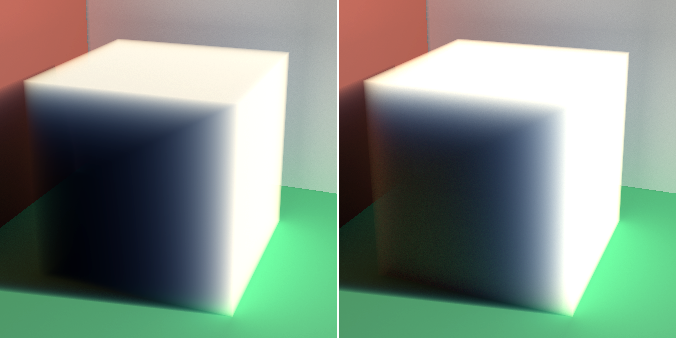
\includegraphics[width=70mm]{../img/inscat_comp2}\\
    }

\end{frame}




%%--------------------------------------------------------------  PCB EXTENSION
\begin{frame}{Sampling the Scene}

    \begin{columns}
        \begin{column}{0.5\textwidth}

    \vspace{-5mm}
    Rays are cast and intersections with objects are recorded\\
    \vspace{8mm}

    Sampling "camera" is behind normal camera with wider field of view\\
    \vspace{8mm}

    \textit{Surfels} are oriented at the intersections aligned along the surface normal

        \end{column}
        \begin{column}{0.5\textwidth}
            \vspace{-4mm}
            \includegraphics[width=\textwidth]{../img/diag/surfel_samp_mod.pdf}\\
        \end{column}
    \end{columns}

\end{frame}




%%--------------------------------------------------------------  PCB EXTENSION
\begin{frame}{Sampling Volumes}

    \begin{columns}
        \begin{column}{0.5\textwidth}

    Samples are taken at discrete steps across the volume domain\\
    \vspace{8mm}

    Scatter/Absorbtion/Lighting factors are averaged within each step\\
    \vspace{8mm}

    \textit{Lvoxels} (spheres) instead of \textit{surfels}

        \end{column}
        \begin{column}{0.5\textwidth}
            \includegraphics[width=\textwidth]{../img/diag/vol_step.pdf}\\
            \vspace{-4mm}
        \end{column}
    \end{columns}

\end{frame}




%%--------------------------------------------------------------  PCB EXTENSION
\begin{frame}{Gathering Light}

    \begin{columns}
        \begin{column}{0.5\textwidth}

    \vspace{-5mm}
    Samples cast into point cloud "gather" light via intersection\\
    \vspace{8mm}

    Samples are returned and used to evaluate the integral over the aligned hemisphere

        \end{column}
        \begin{column}{0.5\textwidth}
            \includegraphics[height=\textwidth]{../img/diag/gather.pdf}\\
            \vspace{-4mm}
        \end{column}
    \end{columns}
    

\end{frame}




%%--------------------------------------------------------------  PCB EXTENSION
\begin{frame}{Integrating Volume Data - Scatter Out}

    \begin{columns}
        \begin{column}{0.5\textwidth}

    Gather stage remains same, no changes necessary\\
    \vspace{8mm}

    Octree must be traversed from back-to-front in order to integrate properly\\
    \vspace{8mm}

    Must keep track of transmittance during traversal

        \end{column}
        \begin{column}{0.5\textwidth}
            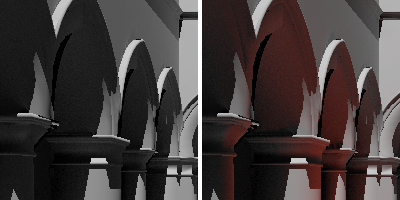
\includegraphics[width=\textwidth]{../img/compare_trad_corrected}\\
            \vspace{2mm}
            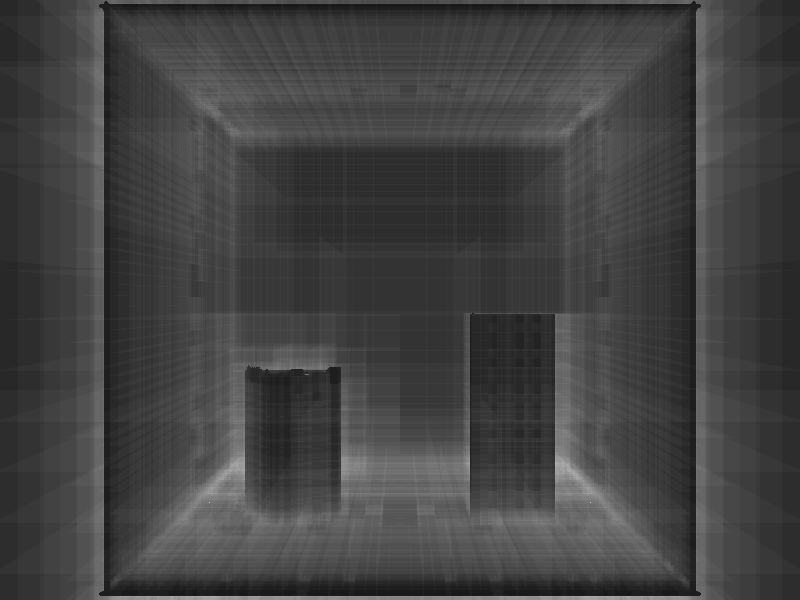
\includegraphics[width=\textwidth]{../img/testing}\\
        \end{column}
    \end{columns}

\end{frame}




%%--------------------------------------------------------------  PCB EXTENSION
\begin{frame}{Integrating Volume Data - Scatter In}

    \begin{columns}
        \begin{column}{0.5\textwidth}

            Modify integration code (normal volume rendering)\\
            \vspace{8mm}

            Add spherical sampling at each volume step\\
            \vspace{8mm}

            For increased performance, attempt full distribution across multiple steps, not at each step

        \end{column}
        \begin{column}{0.5\textwidth}
            \includegraphics[width=\textwidth]{../img/diag/scatter_in.pdf}\\
        \end{column}
    \end{columns}

\end{frame}



%\section{Results}
%%--------------------------------------------------------------------  RESULTS
\begin{frame}{Results - Environment}

    {\bf Test scene involved:}
    \begin{itemize}
        \item 60,000 triangle Sponza Atrium Model\\
        \vspace{2mm}
        \item Stanford CT Scan Data \textit{(Bunny and Head)}
        \vspace{2mm}
    \end{itemize}
    
    {\bf Test run configuration:}
    \begin{itemize}
        \item Run on dual core Intel i5 3.4 GHz, 16 GB machine\\
        \vspace{2mm}
        \item 128 samples per bounce (single bounce)\\
        \vspace{2mm}
        \item 16 samples per in-scatter test\\
        \vspace{2mm}
        \item OpenMP threads split image into vertical chunks for processing\\
    \end{itemize}
\end{frame}




%%--------------------------------------------------------------------  RESULTS
\begin{frame}{Results - Stanford Bunny}

    \begin{changemargin}{-4mm}{0cm}
        \begin{table}
        \begin{center}
        \begin{tabular}{ | l | c | c | c | }
          \hline                       
          Scene & Render Time (s) & Image Delta & Memory Overhead \\

          \hline
          \multicolumn{4}{|c|}{$64^3$ resolution volume} \\     
          \hline            

          Monte Carlo & 3229 sec & NONE & NONE \\
          Traditional PCB & 348 sec & 5.8\% & 466.3 MB (4.780\%) \\
          Extended PCB & 433 sec & 2.1\% & 466.7 MB (4.786\%)  \\

          \hline
          \multicolumn{4}{|c|}{$128^3$ resolution volume} \\     
          \hline            
                     
          Monte Carlo & 3297 sec & NONE & NONE \\
          Traditional PCB & 348 sec & 5.6\% & 466.3 MB (4.780\%) \\
          Extended PCB & 402 sec & 2.4\% & 467.5 MB (4.783\%)  \\

          \hline
          \multicolumn{4}{|c|}{$256^3$ resolution volume} \\     
          \hline            
                     
          Monte Carlo & 3674 sec & NONE & NONE \\
          Traditional PCB & 348 sec & 9.6\% & 466.3 MB (4.780\%) \\
          Extended PCB & 417 sec & 3.8\% & 466.4 MB (4.785\%)  \\
          \hline  

        \end{tabular}
        \caption{Sponza Scene With Stanford Bunny Volume Runtime}
        \end{center}
        \end{table}
    \end{changemargin}

\end{frame}





\begin{frame}{Results - CT Head}

    \begin{changemargin}{-4mm}{0cm}
        \begin{table}
        \begin{tabular}{ | l | c | c | c | }
          \hline                       
          Scene & Render Time (s) & Image Delta & Memory Overhead \\

          \hline
          \multicolumn{4}{|c|}{$64^3$ resolution volume} \\     
          \hline            

          Monte Carlo & 10150 sec & NONE & NONE \\
          Traditional PCB & 348 sec & 14.2\% & 466.3 MB (4.780\%) \\
          Extended PCB & 756 sec & 3.7\% & 468.0 MB (4.800\%)  \\

          \hline
          \multicolumn{4}{|c|}{$128^3$ resolution volume} \\     
          \hline            
                     
          Monte Carlo & 15811 sec & NONE & NONE \\
          Traditional PCB & 348 sec & 14.4\% & 466.3 MB (4.780\%) \\
          Extended PCB & 755 sec & 4.2\% & 467.3 MB (4.790\%)  \\

          \hline
          \multicolumn{4}{|c|}{$256^3$ resolution volume} \\     
          \hline            
                     
          Monte Carlo & 31373 sec & NONE & NONE \\
          Traditional PCB & 348 sec & 14.2\% & 466.3 MB (4.780\%) \\
          Extended PCB & 864 sec & 4.3\% & 467.1 MB (4.790\%)  \\
          \hline  
        \end{tabular}
        \caption{Sponza Scene With CT Head Volume Runtime}
        \end{table}
    \end{changemargin}

\end{frame}



%%-----------------------------------------------------------------  CONCLUSION
\begin{frame}[c]{}

    {\centering
    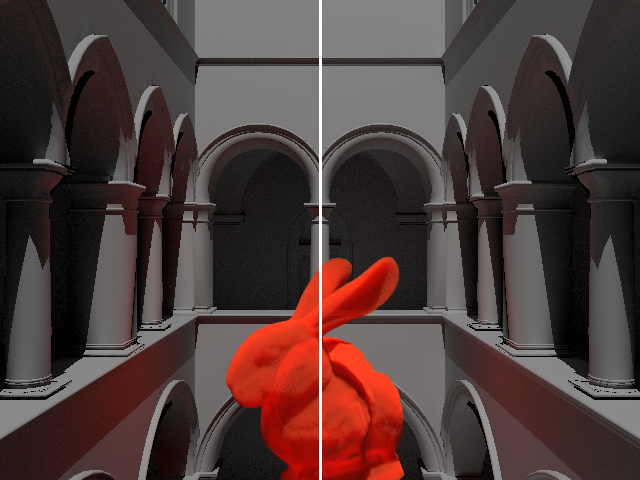
\includegraphics[width=80mm]{../img/compare}\\
    }
    {\centering\scriptsize Comparison of PCBEX results \textit{(left)} and Monte Carlo results \textit{(right)}\\}

\end{frame}




%%-----------------------------------------------------------------  CONCLUSION
\begin{frame}[c]{}

    {\centering
    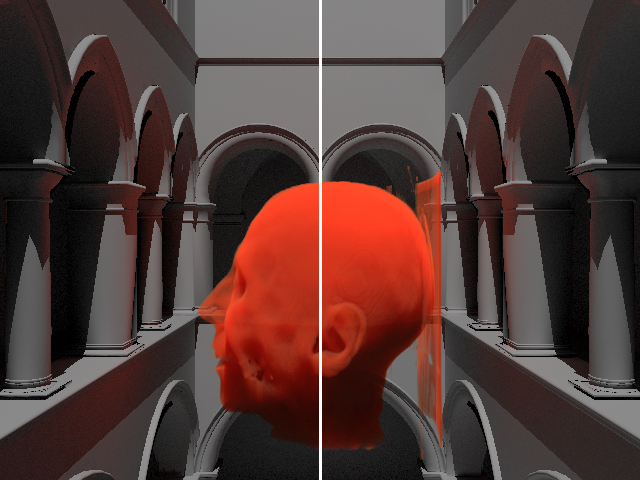
\includegraphics[width=80mm]{../img/compare_head}\\
    }
    {\centering\scriptsize Comparison of PCBEX results \textit{(left)} and Monte Carlo results \textit{(right)}\\}

\end{frame}




%%--------------------------------------------------------------------  RESULTS
\begin{frame}{Image Comparison}


    \begin{columns}
        \begin{column}{0.5\textwidth}
            Close-ups show drastic difference between PCB and PCBEX renders.\\
            \vspace{8mm}
            Full Monte Carlo renders differ only slightly from PCBEX renders.
        \end{column}
        \begin{column}{0.5\textwidth}

            {\centering
            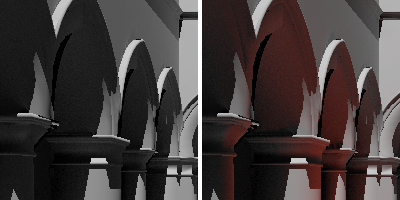
\includegraphics[width=50mm]{../img/compare_trad_corrected}\\
            {\centering\scriptsize PCB vs PCBEX\\}
            
            \vspace{5mm}

            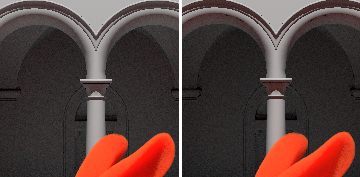
\includegraphics[width=50mm]{../img/compare1_corrected}\\
            {\centering\scriptsize Monte Carlo vs PCBEX\\}
            }
        \end{column}
    \end{columns}


\end{frame}




%%-----------------------------------------------------------------  CONCLUSION
\begin{frame}[c]{}

    \begin{columns}
        \begin{column}{0.5\textwidth}
            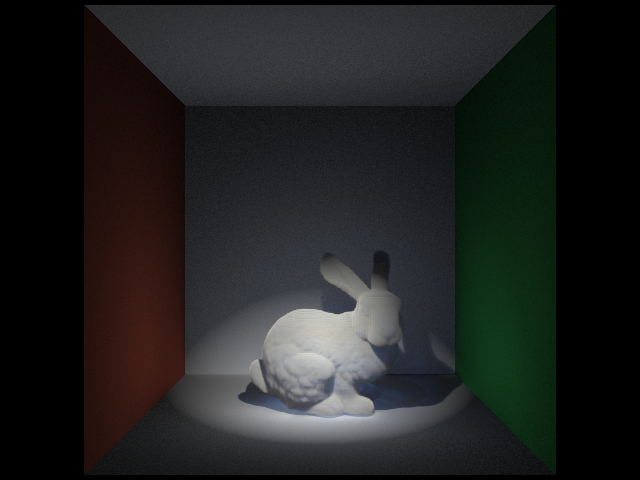
\includegraphics[width=\textwidth]{../img/bunny_spot/spot_front}\\
            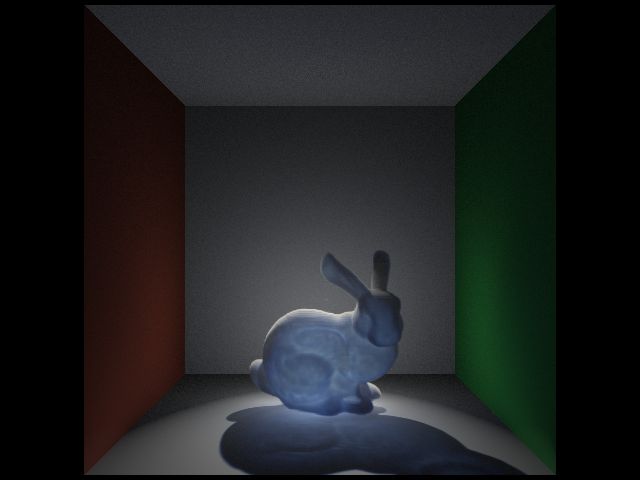
\includegraphics[width=\textwidth]{../img/bunny_spot/spot_behind}\\

        \end{column}
        \begin{column}{0.5\textwidth}
            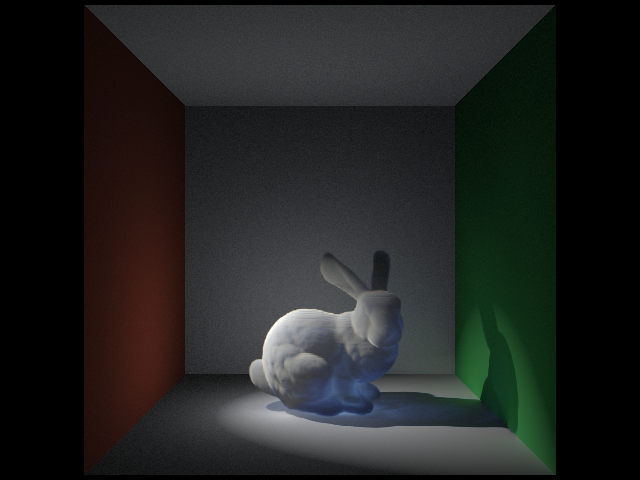
\includegraphics[width=\textwidth]{../img/bunny_spot/spot_left}\\
            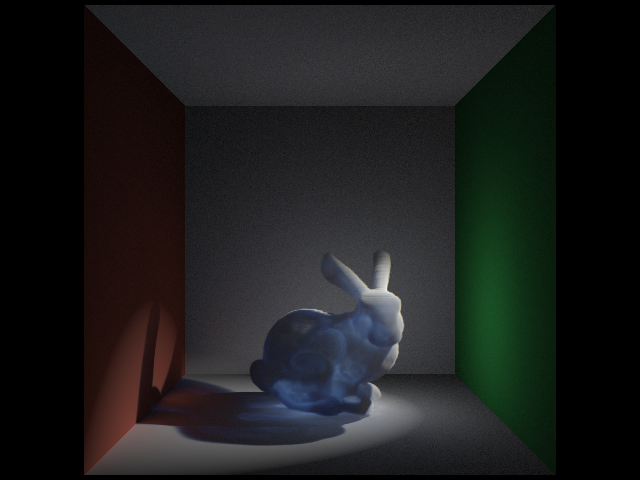
\includegraphics[width=\textwidth]{../img/bunny_spot/spot_right}\\
        \end{column}
    \end{columns}

\end{frame}




%%-----------------------------------------------------------------  CONCLUSION
\begin{frame}[c]{}

    {\centering
    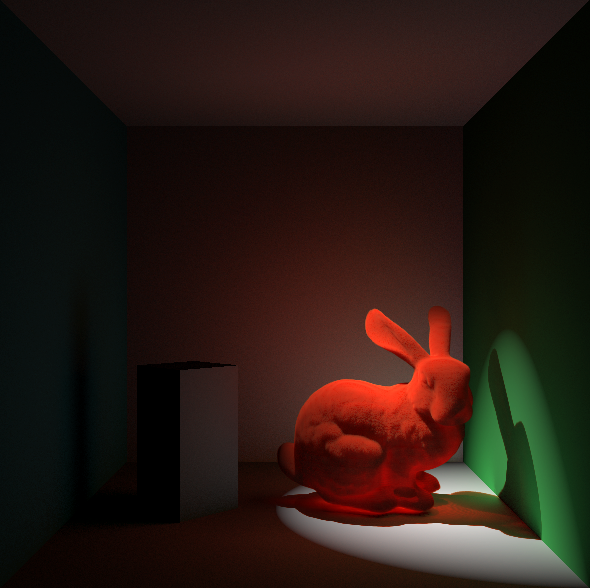
\includegraphics[width=80mm]{../img/ketchup_good_corrected}\\
    }

\end{frame}




%%-----------------------------------------------------------------  CONCLUSION
\begin{frame}[c]{}

    {\centering
    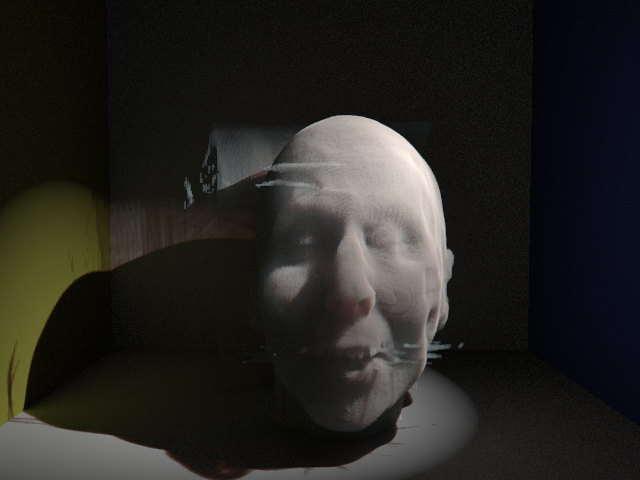
\includegraphics[width=100mm]{../img/face1}\\
    }

\end{frame}




%%-----------------------------------------------------------------  CONCLUSION
\begin{frame}[c]{}

    {\centering
    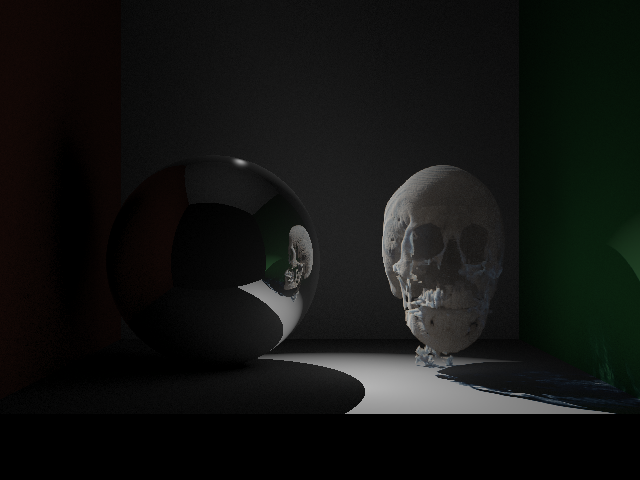
\includegraphics[width=100mm]{../img/sphere_skull}\\
    }

\end{frame}




%%-----------------------------------------------------------------  CONCLUSION
\begin{frame}[c]{}

    {\centering
    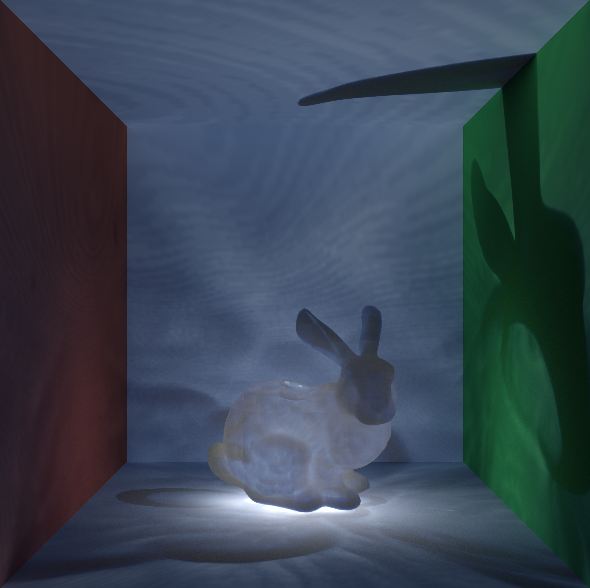
\includegraphics[width=80mm]{../img/bunny_glow}\\
    }

\end{frame}




%%-----------------------------------------------------------------  CONCLUSION
\begin{frame}[c]{}

    {\centering
    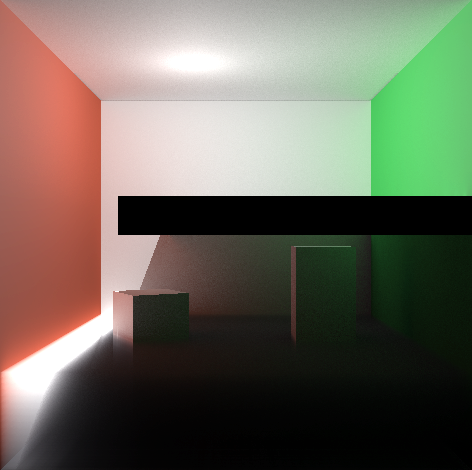
\includegraphics[width=80mm]{../img/one_side_corrected}\\
    }

\end{frame}



%\section{Conclusion}
%%--------------------------------------------------------------------  RESULTS
\begin{frame}{Future Work}

    \begin{enumerate}
        \item Multiple bounce
        \item Phase functions for volumes
        \item Optimal Sampling
    \end{enumerate}

\end{frame}




%%-----------------------------------------------------------------  CONCLUSION
\begin{frame}{Concluding Remarks}

    \begin{columns}
        \begin{column}{0.5\textwidth}

            Modifications can be made to PCB to incorporate volume light contributions\\
            \vspace{8mm}

            Even simple implementations show great improvements in performance, nearly 36 times faster than traditional Monte Carlo\\
            \vspace{8mm}

            Image quality is comparable to Monte Carlo results

        \end{column}
        \begin{column}{0.5\textwidth}
            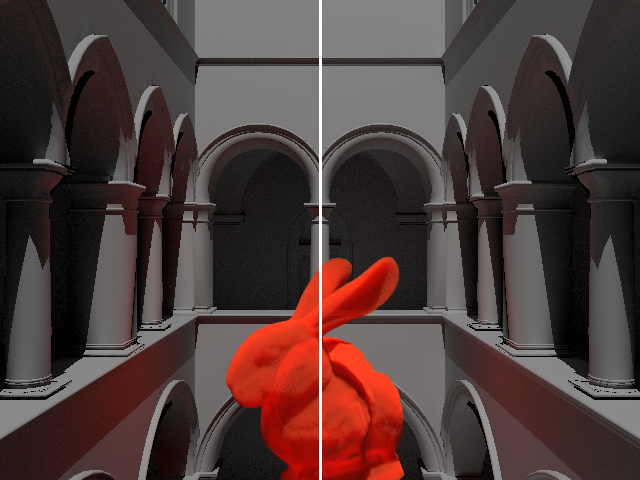
\includegraphics[width=\textwidth]{../img/compare}\\
            {\centering\scriptsize PCBEX \textit{(left)} vs Monte Carlo \textit{(right)} \\}
        \end{column}
    \end{columns}

\end{frame}



%\section{Conclusion}
%%--------------------------------------------------------------------  RESULTS
\begin{frame}{Questions?}

    {\centering Questions?}

\end{frame}




\begin{frame}{Volume Lighting- Phase Functions}


    \begin{columns}
        \begin{column}{0.5\textwidth}

            \begin{block}{Phase Function}
                Described as $phase(w \to w')$
            \end{block}
            \vspace{5mm}

            Describes the probability that light will scatter in any given direction.\\
            \vspace{5mm}
            Used to estimate total scatter-in contribution.

%            \begin{block}{Source Normalization}
%                \[
%                    \int_{\mathbb{S}^2}phase(w \to w')\textup{d}w' = 1.
%                \]
%            \end{block}

        \end{column}
        \begin{column}{0.5\textwidth}
            \vspace{10mm}
            \includegraphics[width=\textwidth]{../img/diag/phase_func_sm}\\
            {\centering\scriptsize Phase function distribution\\}
        \end{column}
    \end{columns}

\end{frame}

\end{document}
